\chapter{Evaluation and Discussion}

\section{Evaluation}

\section{Discussion}

%\section{System Model}\label{sec:system-model}

% TODO - security, privacy, mobile crowd-sensing
% TODO - PDAs vs local computation

%The system model is similar to that in previous work \citep{Ayday2020, Ayday2021}. \Cref{fig:actor-dataflow} illustrates the corresponding data flow\footnote{A \emph{data-flow diagram} consists of data processors (circles), directed data flow (arrows), data stores (parallel lines), and external entities (rectangles) \cite[pp. 437--438]{Fowler2004}\label{foot:dataflow}.}.
%
%\begin{itemize}
%    \item Each user owns a \emph{personal data store} (PDS), a form of cloud storage that empowers the user with ownership and access control over their data.
%    \item Symptom scores are computed in a user's PDS to support integrating multiple streams of personal data \citep{Ayday2020}. While local symptom-score computation \citep{Ayday2020, Ayday2021} is more privacy-preserving, it is assumed that the user's PDS is a trusted entity.
%    \item User device interactions serve as a proxy for proximal human interactions. This work does not assume a specific protocol, but does assume that the protocol can approximate the duration of contact with relative accuracy and that communication with the actors of those contacted users can be established in a privacy-preserving manner.
%    \item No geolocation data is collected \citep{Ayday2020}. As a decentralized, proximity-based solution, it is not necessary to collect user geolocation data. See \Cref{sec:location-based} for a discussion of a geolocation-based design that was considered.
%    \item Actor-based risk propagation is a distributed, online algorithm \cite[pp. 791--818]{Cormen2022}. Previous work \citep{Ayday2020, Ayday2021} (see also \Cref{sec:previous-designs}) formulates risk propagation as a centralized, offline algorithm that periodically aggregates all user data to estimate infection risk. To improve the privacy, scalability, and responsiveness of ShareTrace, this work designs risk propagation to avoid data aggregation and to estimate infection risk in near real-time.
%\end{itemize}
%
%\begin{figure}[htb]
%    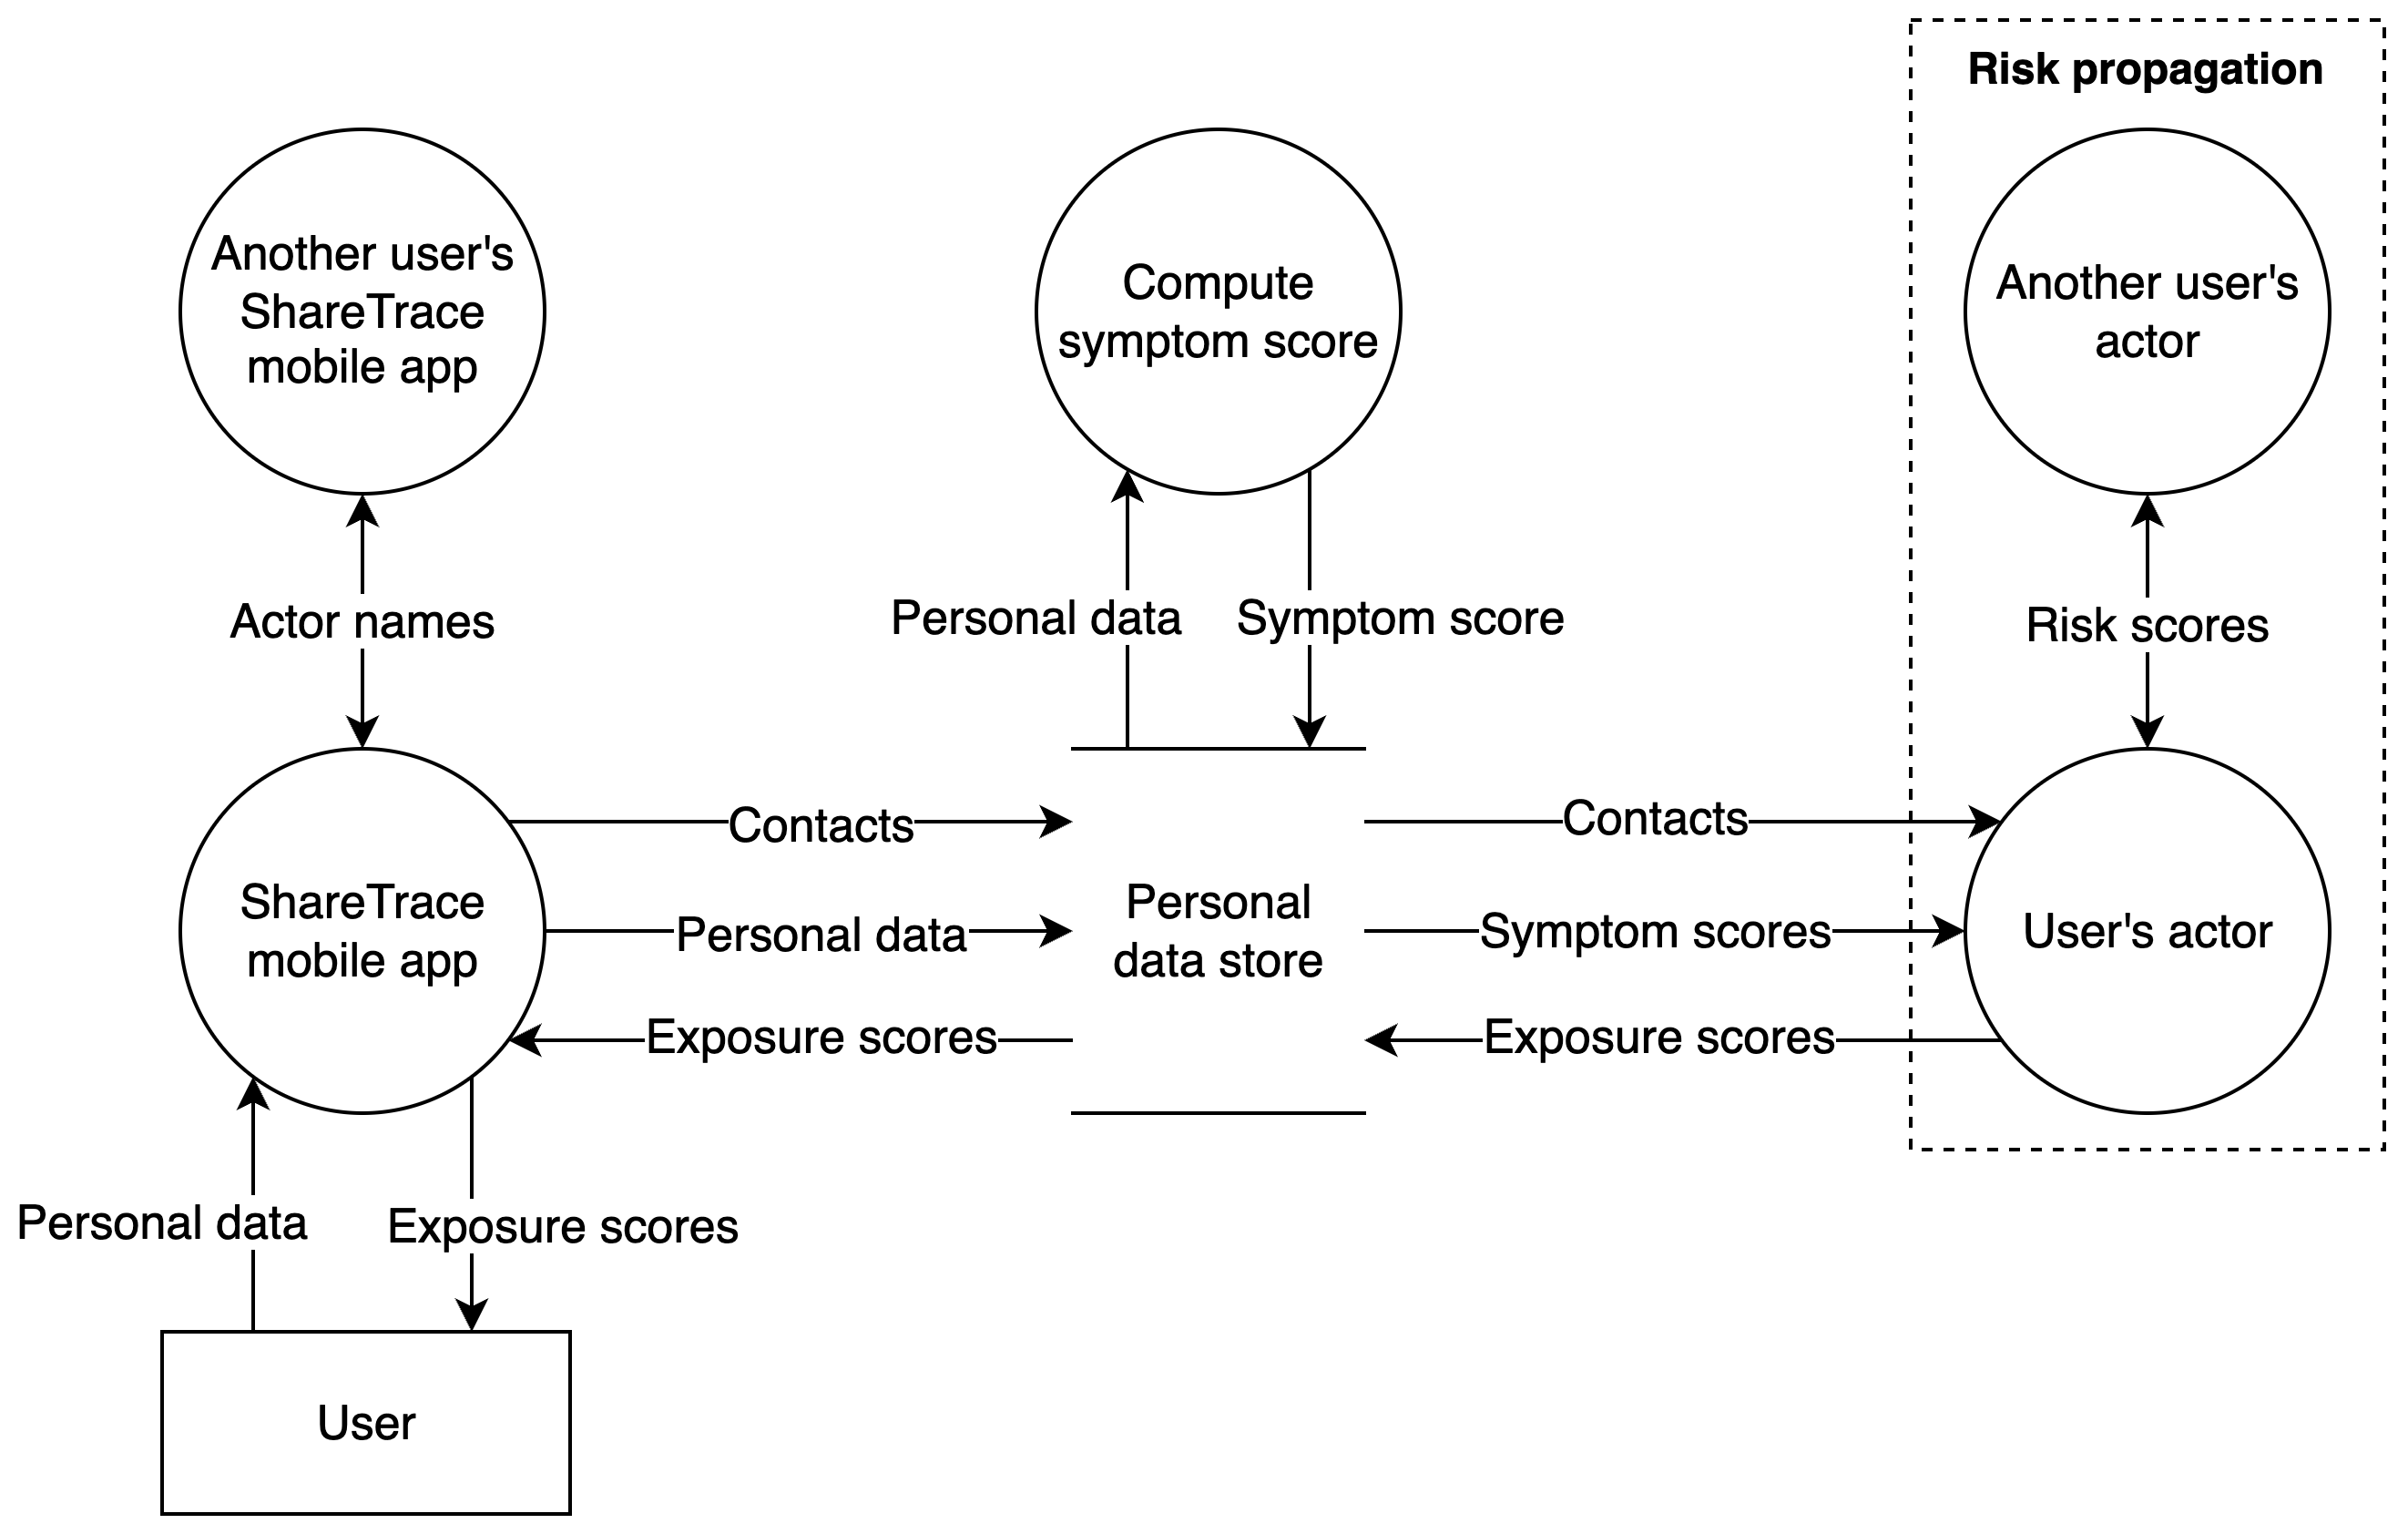
\includegraphics[width=\textwidth]{distributed-dataflow}
%    \caption[Distributed ShareTrace data flow]{Distributed ShareTrace data flow. \emph{Contacts} include the actor name and contact time of all users with which the user came into close proximity. \emph{Personal data} includes the user's demographics, reported symptoms, and diagnosis. It may also include machine-generated biomarkers and electronic health record data \citep{Ayday2020}.}
%    \label{fig:distributed-dataflow}
%\end{figure}
%
%\begin{figure}[htb]
%    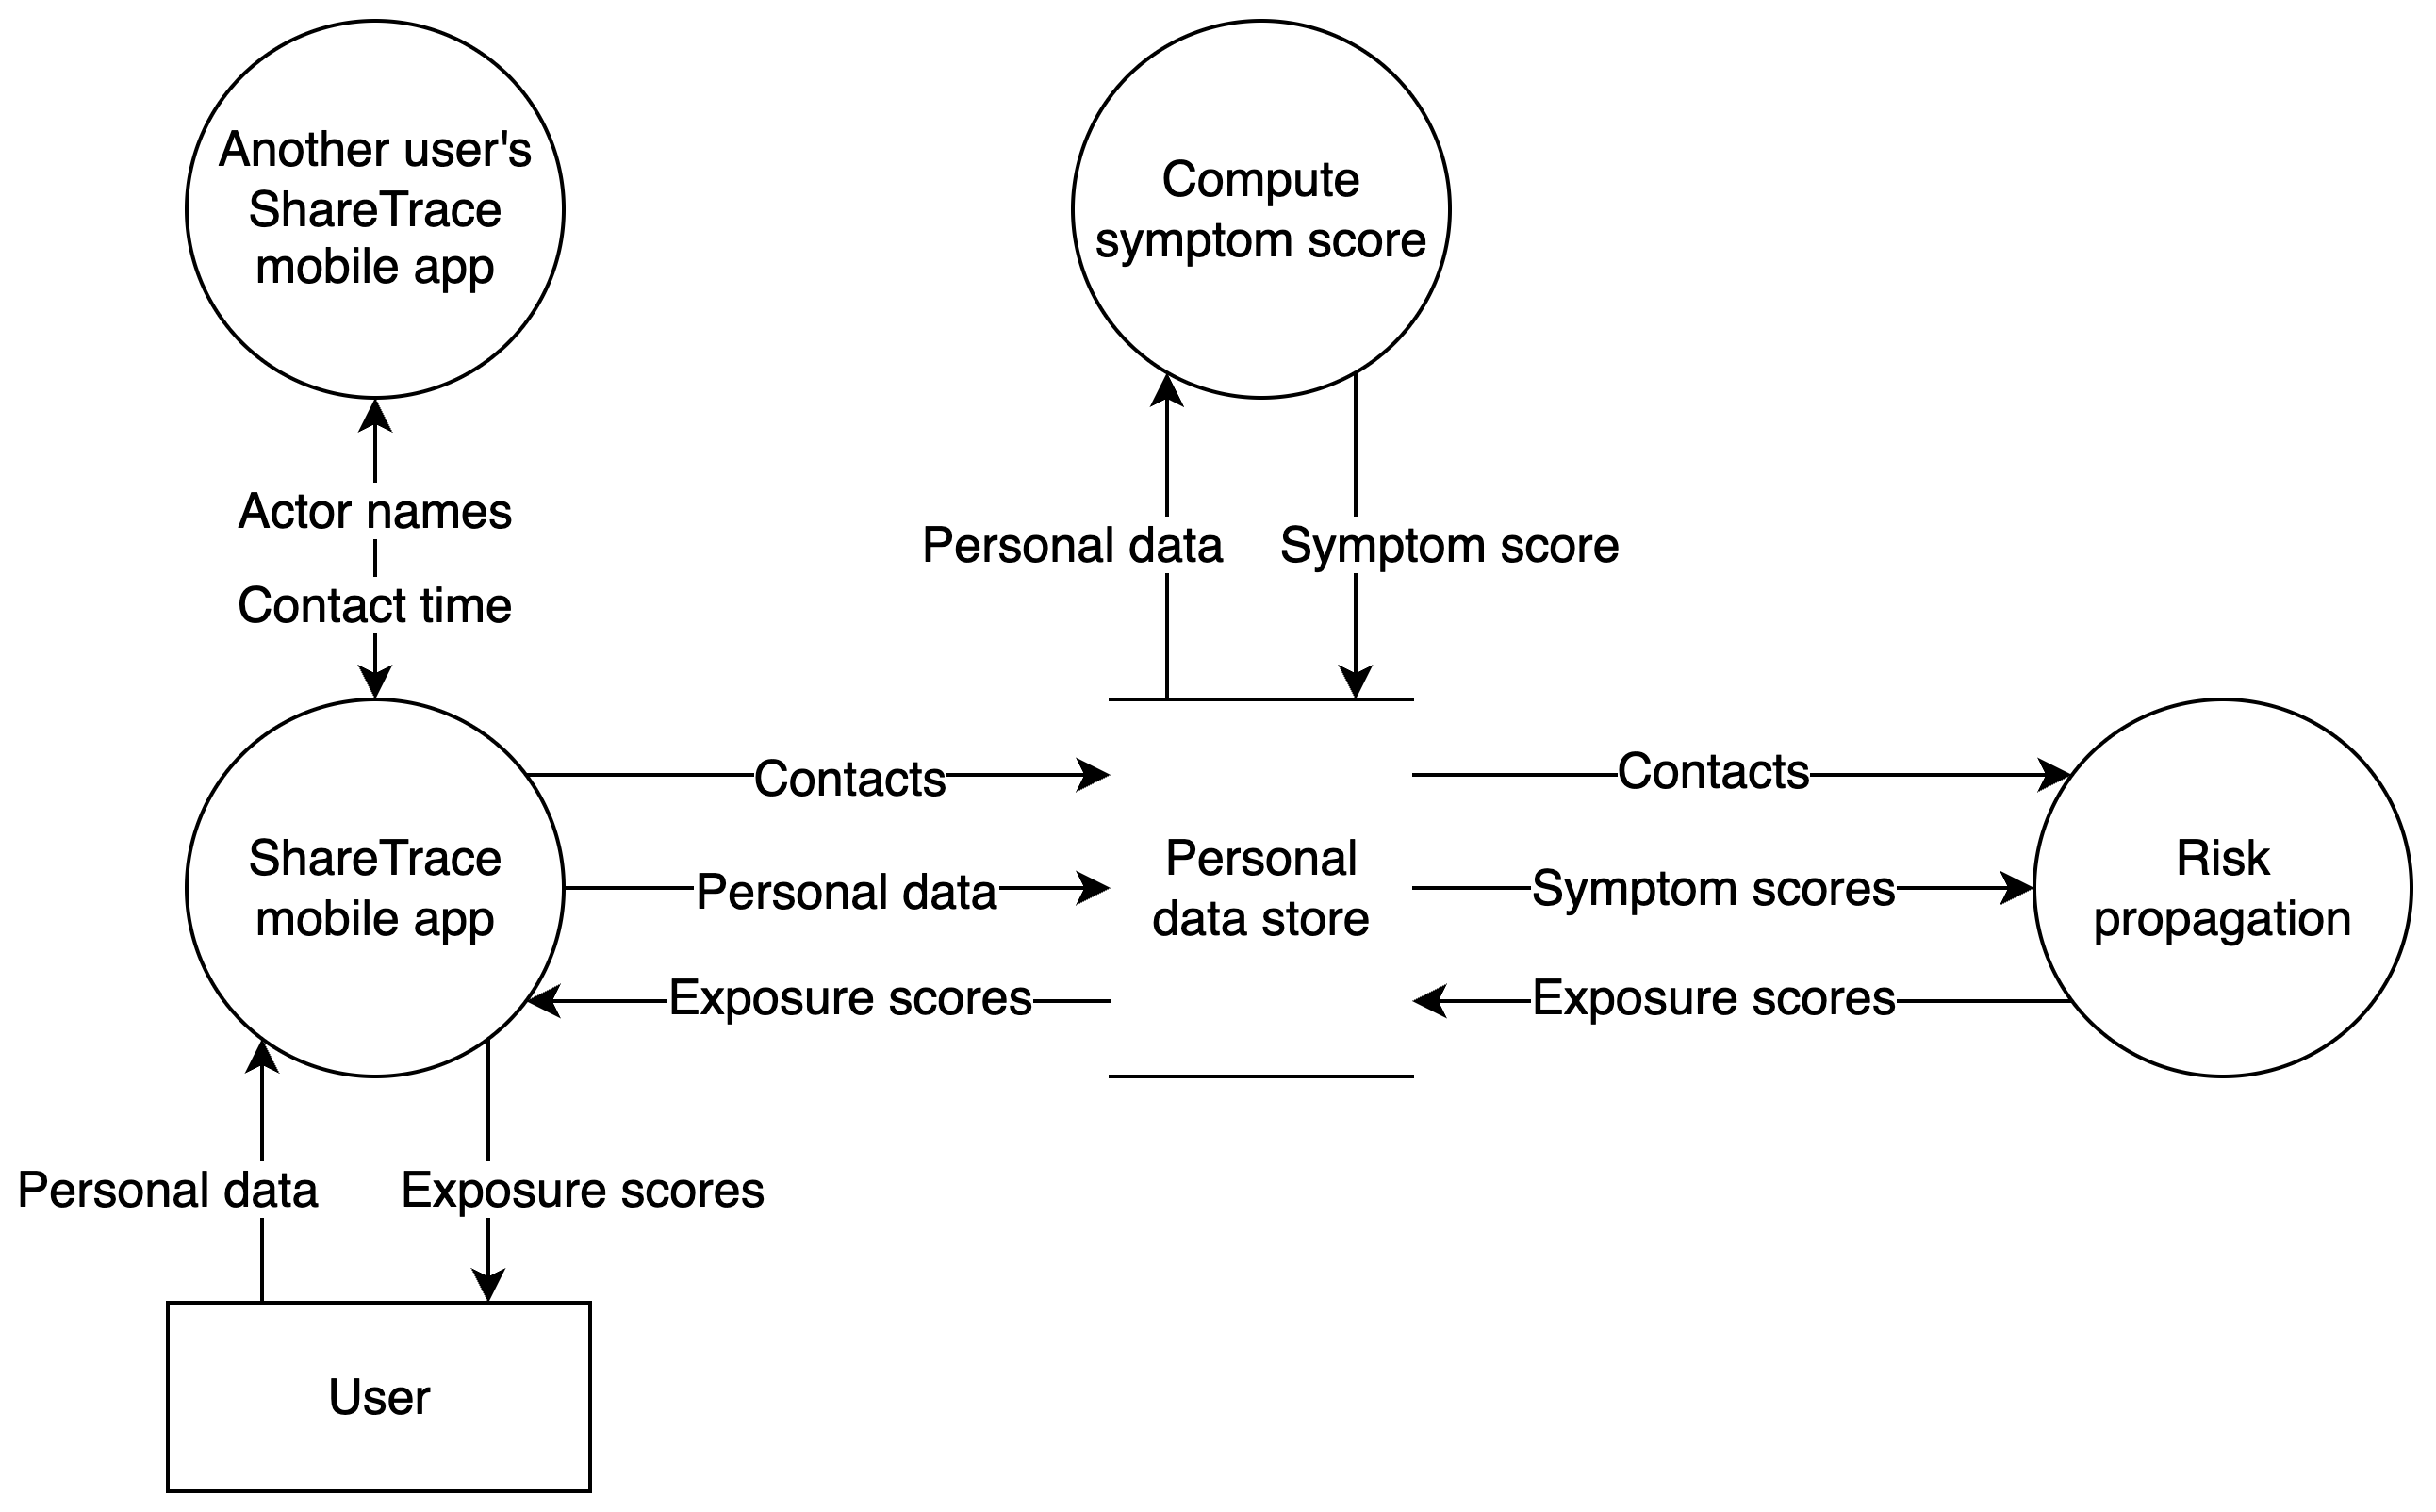
\includegraphics[width=\textwidth]{centralized-dataflow}
%    \caption[Centralized ShareTrace data flow]{Centralized ShareTrace data flow. \emph{Contacts} include the actor name and contact timestamp of all users with which the user came into close proximity. \emph{Personal data} includes the user's demographics, reported symptoms, and diagnosis. It may also include machine-generated biomarkers and electronic health record data \citep{Ayday2020}.}
%    \label{fig:centralized-dataflow}
%\end{figure}

\subsection{Mobile Crowdsensing}

\define{Mobile crowdsensing} (MCS) is a ``sensing paradigm that empowers ordinary citizens to contribute data sensed or generated from their mobile devices'' that is aggregated  ``in the cloud for crowd intelligence extraction and human-centric service delivery'' \cite{Guo2015}. Over the past decade, substantial research has been conducted on defining and classifying MCS applications \cite[and references therein]{Capponi2019, Guo2015}. While not discussed in previous work \cite{Ayday2020, Ayday2021}, ShareTrace is a MCS application. The following characterization of ShareTrace assumes the four-layered architecture of a MCS application \cite{Capponi2019}, which offers a comprehensive set of classification criteria that To offer a clear comparison, \Cref{tab:classification} follows the same structure as \cite{Capponi2019}. Some aspects of the architecture, namely sampling frequency and sensor activity, are marked according to how ShareTrace is described in previous work, rather than how it would function to optimize for energy efficiency. More detail is provided below in this regard. When classifying ShareTrace as an MCS application, the following description is helpful:
%
\begin{quote}
	\emph{ShareTrace is a decentralized, delay-tolerant contact-tracing application that estimates infection risk from proximal user interactions and user symptoms.}
\end{quote}

\subsubsection{Application Layer}

\paragraph{Application Tasks}

\subparagraph{Task Scheduling}

\emph{Proactive scheduling} allows users to decide when and where they contribute sensing data, while \emph{reactive scheduling} requires that ``a user receives a request, and upon acceptance, accomplishes a task'' \cite{Capponi2019}. ShareTrace follows proactive scheduling where the sensing task is to detect proximal interactions with other users. Naturally, the scheduling of this task is at the discretion of the ShareTrace user.

\subparagraph{Task Assignment}

\emph{Centralized assignment} assumes that ``a central authority distributes tasks among users.'' Conversely, with \emph{decentralized assignment}, ``each participant becomes an authority and can either perform the task or forward it to other users. This approach is very useful when users are very interested in specific events or activities'' \cite{Capponi2019}. The latter naturally aligns with ShareTrace in which each user is responsible for their own interactions that are both temporally and spatially specific.

\subparagraph{Task Execution}

With \emph{single-task execution}, MCS applications assign one type of task to users, while \emph{multi-task execution} assigns  multiple types of tasks \cite{Capponi2019}. ShareTrace only involves the single task of sensing proximal interactions. Alternatively, ShareTrace could be defined more abstractly as sensing infection risk through interactions and user symtpoms. In this case, ShareTrace would follow a multi-tasked execution model, where the task of sensing user symptoms is achieved through user reporting or bodily sensors.

\paragraph{Application Users}

\subparagraph{User Recruitment}

\emph{Volunteer-based recruitment} is when citizens can ``join a sensing campaign for personal interests{\ldots}or willingness to help the community,'' while \emph{incentive-based recruitment} promotes participation and offers control over the recruitment rate{\ldots}These strategies are not mutually exclusive and users can first volunteer and then be rewarded for quality execution of sensing tasks'' \cite{Capponi2019}. ShareTrace assumes volunteer-based recruitment. However, as a decentralized application (dApp) that aligns with the principles of self-sovereignty, an incentive structure that rewards users with verifiable, high-quality data is plausible.

\subparagraph{User Selection}

\emph{User-centric selection} is when ``contributions depend only on participants['] willingness to sense and report data to the central collector, which is not responsible for choosing them.'' \emph{Platform-centric selection} is ``when the central authority directly decides data contributors{\ldots}Platform centric decisions are taken according to the utility of data to accomplish the targets of the campaign'' \cite{Capponi2019}. ShareTrace employs user-centric selection, because the purpose of the application is to passively sense the user's interactions and provide them with the knowledge of their infection risk.

\subparagraph{User Type}

A \emph{contributor} ``reports data to the MCS platform with no interest in the results of the sensing campaign'' and ``are typically driven by incentives or by the desire to help the scientific or civil communities.'' A \emph{consumer} joins ``a service to obtain information about certain application scenario[s] and have a direct interest in the results of the sensing campaign'' \cite{Capponi2019}. For ShareTrace, users can be either a consumer or a contributor but are likely biased toward the former.

\subsubsection{Data Layer}

\paragraph{Data Management}

\subparagraph{Data Storage}

\emph{Centralized storage} involves data being ``stored and maintained in a single location, which is usually a database made available in the cloud. This approach is typically employed when significant processing or data aggregation is required.'' \emph{Distributed storage} ``is typically employed for delay-tolerant applications, i.e., when users are allowed to deliver data with a delayed reporting'' \cite{Capponi2019}. For sensing human interaction, ShareTrace relies on distributed storage in the form of Dataswift Personal Data Accounts. Moreover, ShareTrace is delay-tolerant, so distributed storage is most appropriate. However, for reporting the population-level risk distribution, it is likely that centralized storage would be used.

\subparagraph{Data Format}

\emph{Structured data} is standardized and readily analyzable. \emph{Unstructured data}, however, requires significant processing before it can be used \cite{Capponi2019}. ShareTrace deals with structured data (e.g., user symptoms, actor URIs).

\subparagraph{Data Dimensionality}

\emph{Single-dimension data} typically occurs when a single sensor is used, while \emph{multi-dimensional data} arises with the use of multiple sensors. ShareTrace data is one-dimensional because it only uses Bluetooth to sense nearby users.

\paragraph{Data Processing}

\subparagraph{Data Pre-processing}

\emph{Raw data output} implies that no modification is made to the sensed data. \emph{Filtering and denoising} entail ``removing irrelevant and redundant data. In addition, they help to aggregate and make sense of data while reducing at the same time the volume to be stored'' \cite{Capponi2019}. ShareTrace only retains the actor URIs that correspond to valid contacts (i.e., lasting at least 15 minutes).

\subparagraph{Data Analytics}

\emph{Machine learning} (ML) \emph{and data mining analytics} are not real-time. They ``aim to infer information, identify patterns, or predict future trends.'' On the contrary, \emph{real-time analytics} consist of ``examining collected data as soon as it is produced by the contributors'' \cite{Capponi2019}. ShareTrace aligns with the former category since it aims to infer the infection risk of users.

\subparagraph{Data Post-processing}

\emph{Statistical post-processing} ``aims at inferring proportions given quantitative examples of the input data. \emph{Prediction post-processing} aims to determine ``future outcomes from a set of possibilities when given new input in the system'' \cite{Capponi2019}. ShareTrace applies predictive post-processing via risk propagation.

\subsubsection{Communication Layer}

\paragraph{Communication Technology}

\subparagraph{Infrastructured Technology}

\emph{Cellular} connectivity ``is typically required from sensing campaign[s] that perform real-time monitoring and require data reception as soon as it is sensed.'' \emph{WLAN} ``is used mainly when sensing organizers do not specify any preferred reporting technologies or when the application domain permits to send data'' at ``a certain amount of time after the sensing process'' \cite{Capponi2019}. Infrastructured technology is also referred to as the \emph{infrastructured transmission paradigm} \cite{Ma2014}. ShareTrace does not require cellular infrastructure, because it is delay-tolerant and thus only requires WLAN.

\subparagraph{Infrastructure-less Technology}

\emph{Infrastructure-less technologies} ``consists of device-to-device (D2D) communications that do not require any infrastructure{\ldots}but rather allow devices in the vicinity to communicate directly.'' Technologies include \emph{WiFi-Direct}, \emph{LTE-Direct}, and \emph{Bluetooth} \cite{Capponi2019}. Infrastructure-less technology is also called the \emph{opportunistic transmission paradigm} \cite{Ma2014}. ShareTrace uses Bluetooth because of its energy efficiency and short range.

\paragraph{Data Reporting}

\subparagraph{Upload mode}

With \emph{relay uploading}, ``data is delivered as soon as collected.'' \emph{Store-and-forward} ``is typically used in delay-tolerant applications when campaigns do not need to receive data in real-time'' \cite{Capponi2019}. Because ShareTrace is delay-tolerant, it uses store-and-forward uploading.

\subparagraph{Metholodgy}

\emph{Individualized sensing} is ``when each user accomplishes the requested task individually and without interaction with other participants.'' \emph{Collaborative sensing} is when ``users communicate with each other, exchange data[,] and help themselves in accomplishing a task or delivering information to the central collector. Users are typically grouped and exchange data exploiting short-range communication technologies, such as WiFi-[D]irect or Bluetooth{\ldots}Note that systems that create maps merging data from different users are considered individual because users do not interact between each other to contribute'' \cite{Capponi2019}. The methodology of sensing is similar to the \emph{sensing scale} which is typically dichotomized as \emph{personal} \cite{Lane2010, Ganti2011} (i.e., individualized) and \emph{community} \cite{Ganti2011} or \emph{group} \cite{Lane2010} (i.e., collaborative). ShareTrace is inherently collaborative, relying on mobile devices to exchange actor URIs to estimate infection risk. Thus, collaborative sensing is used.

\subparagraph{Timing}

\emph{Timing} is based on whether devices ``should sense in the same period or not.'' \emph{Synchronous timing} ``includes cases in which users start and accomplish at the same time the sensing task. For synchronization purposes, participants communicate with each other.'' \emph{Asynchronous timing} occurs ``when users perform sensing activity not in time synchronization with other users'' \cite{Capponi2019}. ShareTrace requires synchronous timing, because contact sensing inherently requires synchronous communication between the involved devices.

\subsubsection{Sensing Layer}

\paragraph{Sensing Elements}

\subparagraph{Sensor Deployment}

\emph{Dedicated deployment} involves the use of ``non-embedded sensing elements,'' typically for a specific task. \emph{Non-dedicated deployment} utilizes sensors that ``do not require to be paired with other devices for data delivery but exploit the communication capabilities of mobile devices'' \cite{Capponi2019}. ShareTrace relies on non-dedicated deployment since it relies on Bluetooth that is ubiquitous in modern-day mobile devices.

\subparagraph{Sensor Activity}

\emph{Always-on sensors} ``are required to accomplish mobile devices['] basic functionalities, such as detection of rotation and acceleration{\ldots} Activity recognition [i.e., context awareness]{\ldots}is a very important feature that accelerometers enable.'' \emph{On-demand sensors} ``need to be switched on by users or exploiting an application running in the background. Typically, they serve more complex applications than always-on sensors and consume a higher amount fo energy'' \cite{Capponi2019}. ShareTrace uses Bluetooth, which may be considered on-demand. While energy efficient, users do control when it is enabled. Ideally, ShareTrace would also use always-on sensors to enable Bluetooth with context awareness (i.e., that the user is carrying or nearby the device).

\subparagraph{Acquisition}

\emph{Homogeneous acquisition} ``involves only one type of data and it does not change from one user to another one,'' while \emph{heterogeneous acquisition} ``involves different data types usually sampled from several sensors'' \cite{Capponi2019}. ShareTrace is homogeneous, because all users sense the same data from one type of sensor.

\paragraph{Data Sampling}

\subparagraph{Sampling Frequency}

\emph{Continuous sensing} ``indicates tasks that are accomplished regularly and independently [of] the context of the smartphone or the user['s] activities.'' \emph{Event-based sensing} is ``data collection [that] starts after a certain event has occurred. In this context, an event can be seen as an active action from a user or the central collector, but also a given context awareness'' \cite{Capponi2019}. ShareTrace sensing is continuous but would ideally be event-based to conserve device energy.

\subparagraph{Sensing Responsibility}

When the \emph{mobile device} is responsible, ``devices or users take sampling decisions locally and independently from the central authority{\ldots}When devices take sampling decisions, it is often necessary to detect the context [of the] smartphones and wearable devices{\ldots}The objective is to maximize the utility of data collection and minimize the cost of performing unnecessary operations.'' When the \emph{central collector} is responsible, they make ``decisions about sensing and communicate them to the mobile devices'' \cite{Capponi2019}. Given the human-centric nature of the ShareTrace sensing task, mobile devices are responsible.

\subparagraph{User involvement}

\emph{Participatory involvement} ``requires active actions from users, who are explicitly asked to perform specific tasks. They are responsible to consciously meet the application requests by deciding when, what, where, and how to perform sensing tasks.'' \emph{Opportunistic involvement} means that ``users do not have direct involvement, but only declare their interest in joining a campaign and providing their sensors as a service. Upon a simple handshake mechanism between the user and the MCS platform, a MCS thread is generated on the mobile device (e.g., in the form of a mobile app), and the decisions of what, where, when, and how to perform the sensing are delegated to the corresponding thread. After having accepted the sensing process, the user is totally unconscious with no tasks to perform and data collection is fully automated{\ldots}The smartphone itself is context-aware and makes decisions to sense and store data, automatically determining when its context matches the requirements of an application. Therefore, coupling opportunistic MCS systems with context-awareness is a crucial requirement'' \cite{Capponi2019}. Earlier works on MCS refer to user involvement as the \emph{sensing paradigm} \cite{Lane2010, Ganti2011, Ma2014}. ShareTrace is opportunistic, ideally with context-awareness.

\begin{table}[htb]
\renewcommand{\arraystretch}{0.85}
\scriptsize
\centering
\begin{tabularx}{\textwidth}{
    >{\centering\arraybackslash}X
    >{\centering\arraybackslash}X
    >{\centering\arraybackslash}X
    c
    >{\centering\arraybackslash}X}
\toprule
\multirow{12}*{Application}
	& \multirow{6}*{Task}
		& \multirow{2}*{Scheduling}
			& Proactive & $\bullet$ \\
			&&& Reactive & \\
		\cmidrule{3-5}
		&& \multirow{2}*{Assignment}
			& Centralized & \\
			&&& Decentralized & $\bullet$ \\
		\cmidrule{3-5}
		&& \multirow{2}*{Execution}
			& Single task & $\bullet$ \\
			&&& Multi-tasking & \\
	\cmidrule{2-5}
	& \multirow{6}*{User}
		& \multirow{2}*{Recruitment}
			& Voluntary & $\bullet$ \\
			&&& Incentivized & \\
		\cmidrule{3-5}
		&& \multirow{2}*{Selection}
			& Platform-centric & \\
			&&& User-centric & $\bullet$ \\
		\cmidrule{3-5}
		&& \multirow{2}*{Type}
			& Consumer & $\bullet$ \\
			&&& Contributor & $\bullet$ \\
		\cmidrule{2-5}
\cmidrule{1-5}
\multirow{12}*{Data}
	& \multirow{6}*{Management}
		& \multirow{2}*{Storage}
			& Centralized & \\
			&&& Distributed & $\bullet$ \\
		\cmidrule{3-5}
		&& \multirow{2}*{Format}
			& Structured & $\bullet$ \\
			&&& Unstructured & \\
		\cmidrule{3-5}
		&& \multirow{2}*{Dimension}
			& Single dimension & $\bullet$ \\
			&&& Multi-dimensional & \\
	\cmidrule{2-5}
	& \multirow{6}*{Processing}
		& \multirow{2}*{Pre-processing}
			& Raw data & \\
			&&& Filtering and denoising & $\bullet$ \\
		\cmidrule{3-5}
		&& \multirow{2}*{Analytics}
			& ML and data mining & $\bullet$ \\
			&&& Real-time & \\
		\cmidrule{3-5}
		&& \multirow{2}*{Post-processing}
			& Statistical & \\
			&&& Prediction & $\bullet$ \\
		\cmidrule{2-5}
\cmidrule{1-5}
\multirow{11}*{Communication}
	& \multirow{5}*{Technologies}
		& \multirow{2}*{Infrastructured}
			& Cellular & $\bullet$ \\
			&&& WLAN & $\bullet$ \\
		\cmidrule{3-5}
		&& \multirow{3}*{Infrastructure-less}
			& LTE-Direct & \\
			&&& WiFi-Direct & \\
			&&& Bluetooth & $\bullet$ \\
		\cmidrule{3-5}
	\cmidrule{2-5}
	& \multirow{6}*{Reporting}
		& \multirow{2}*{Upload mode}
			& Relay & \\
			&&& Store and forward & $\bullet$ \\
		\cmidrule{3-5}
		&& \multirow{2}*{Methodology}
			& Individual & \\
			&&& Collaborative & $\bullet$ \\
		\cmidrule{3-5}
		&& \multirow{2}*{Timing}
			& Synchronous & $\bullet$ \\
			&&& Asynchronous & \\
		\cmidrule{2-5}
\cmidrule{1-5}
\multirow{12}*{Sensing}
	& \multirow{6}*{Elements}
		& \multirow{2}*{Deployment}
			& Dedicated & \\
			&&& Non-dedicated & $\bullet$ \\
		\cmidrule{3-5}
		&& \multirow{2}*{Activity}
			& Always-on & $\bullet$ \\
			&&& On-demand & $\circ$ \\
		\cmidrule{3-5}
		&& \multirow{2}*{Acquisition}
			& Homogeneous & $\bullet$ \\
			&&& Heterogeneous & \\
	\cmidrule{2-5}
	& \multirow{6}*{Sampling}
		& \multirow{2}*{Frequency}
			& Continuous & $\bullet$ \\
			&&& Event-based & $\circ$ \\
		\cmidrule{3-5}
		&& \multirow{2}*{Responsibility}
			& Mobile device & $\bullet$ \\
			&&& Central collector & \\
		\cmidrule{3-5}
        && \multirow{2}*{User involvement}
			& Participatory & \\
			&&& Opportunistic & $\bullet$ \\
\bottomrule
\end{tabularx}
\caption[ShareTrace classification]{ShareTrace classification using the four-layered architecture of a mobile crowdsensing application \cite{Capponi2019}. Always ($\bullet$); with context-awareness ($\circ$).}
\label{tab:classification}
\end{table}

\clearpage

\subsection{Self-Sovereignty}